
\chapter{Hynesim}
\label{chap:hynesim}

Firstly, we will present Hynesim. I fact, we will use this tool to create all our network and test our solution so
it is important to introduce it.

\section{Presentation}

\begin{figure}[h]
  \centering
  
\includegraphics[width=0.5\textwidth]{hynesim}
  \caption{Hynesim logo}
  \label{fig:hynesim}
\end{figure}


\definition{Hynesim}{Means HYbrid NEtwork SIMulation, is a distribute platform of simulation of information system
  developed by Diateam. \cite{hynesim}}

The platform was initially developed by Diateam for DGA MI (Maitrise de l'information) to create virtual network.
But now is a major project to develop information system and automatize cyber security attacks. This project has
two version, an open source version and an professional version. The open source version as less option, but we
will use this version for this project.

\section{Architecture}

To work, Hynesim need a server with on it the main software. This software is the virtualization part. It manage
virtual machine and network.

Moreover, to see virtual machine and interact with them, users need to have the client interface. This interface
can be install on a simple computer.

\begin{figure}[h]
  \centering
  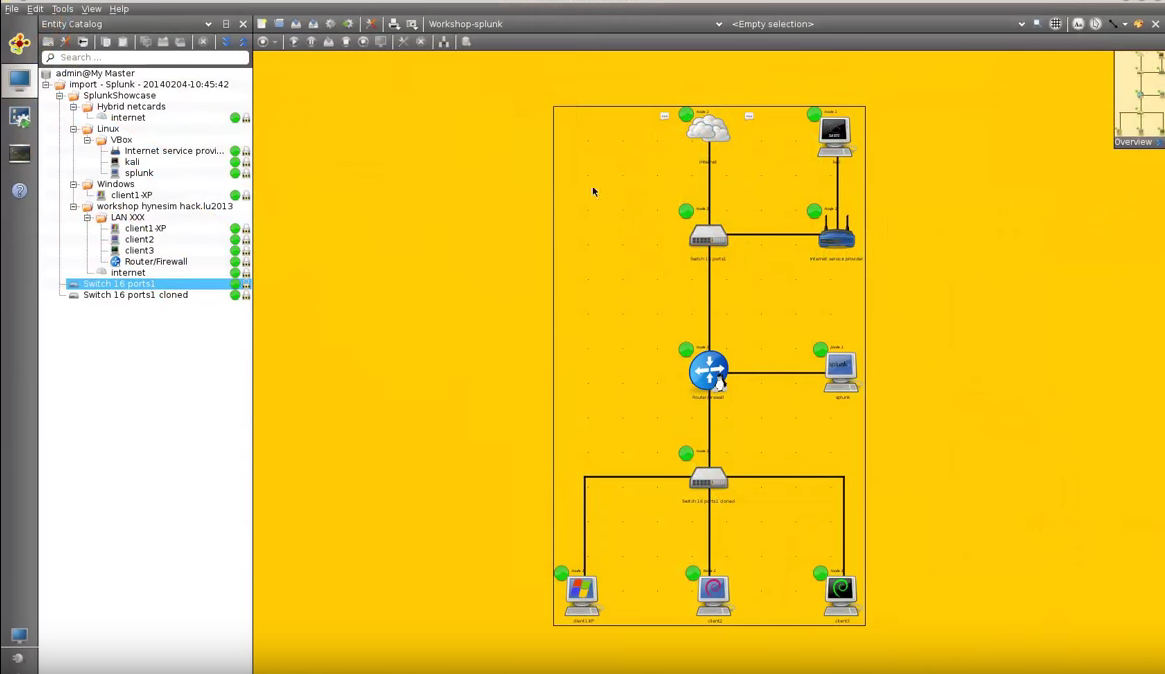
\includegraphics[width=\textwidth]{hynesim_network}
  \caption{An example of an hynesim network}
\end{figure}





%%% Local Variables:
%%% mode: latex
%%% TeX-master: "../rapport_de_base"
%%% End:
